\documentclass{homework}
\usepackage{setspace}
\onehalfspacing
\usepackage{float}
\usepackage{needspace}
% \Needspace{10\baselineskip}  % adjust based on expected box height
\usepackage{placeins}
\FloatBarrier
\usepackage{fvextra}
\usepackage{minted} % for code highlighting
\usepackage[most]{tcolorbox}
\tcbuselibrary{listings, minted, breakable}
\usepackage{hyperref}
\usepackage{nameref}
\usepackage[utf8]{inputenc}
\usepackage{newunicodechar}


% Greek Letters
\newunicodechar{ν}{\ensuremath{\nu}}        % Poisson's ratio
\newunicodechar{μ}{\ensuremath{\mu}}        % Shear modulus
\newunicodechar{λ}{\ensuremath{\lambda}}    % Lamé parameter
\newunicodechar{σ}{\ensuremath{\sigma}}     % Stress
\newunicodechar{ε}{\ensuremath{\varepsilon}} % Strain
\newunicodechar{Ω}{\ensuremath{\Omega}}     % Domain/Triangulation
\newunicodechar{Γ}{\ensuremath{\Gamma}}     % Boundary

% Math Operators & Symbols
\newunicodechar{∫}{\ensuremath{\int}}       % Integral symbol
\newunicodechar{⋅}{\ensuremath{\cdot}}      % Dot product
\newunicodechar{⊙}{\ensuremath{\odot}}      % Double contraction
\newunicodechar{∘}{\ensuremath{\circ}}      % Composition


\author{Shivam Kumar}
\class{Roll. No.: 22CE01046}
\date{\today}
\title{Assignment-2 (CAD Laboratory)}
% \address{CAD Laboratory}

% ---------- Colors ----------
\definecolor{pbheader}{RGB}{240,240,240}   % header background
\definecolor{framecol}{RGB}{190,190,190}   % frame color  
\definecolor{solcol}{RGB}{230,240,250}
\definecolor{mybg}{RGB}{245,245,230}

% ---------- Solution environment ----------
\newtcolorbox{solution}{
  enhanced,
  breakable,
  sharp corners=all,
  colframe=framecol,
  colback=solcol,
  left=6pt, right=6pt, top=6pt, bottom=6pt,
  boxrule=0.5pt,
  before skip=6pt,
  after skip=12pt,
  fonttitle=\bfseries,
  borderline west={2pt}{0pt}{pbheader}
}

% % % Configure minted for Julia
\setminted[julia]{
    linenos,          % show line numbers
    breaklines,      % wrap long lines
    breakanywhere,
    breakautoindent=true,
    fontsize=\small,  % smaller font
    bgcolor=mybg,     % light gray background
    frame=none,          % frame around code
    numbersep=5pt,        % space between line numbers and code
    xleftmargin=10pt      % left margin
}

\graphicspath{{./media/}}

\begin{document} \maketitle


\hrule

\question Given the two-dimensional body
\[ \mathcal{B}=\{(X_{1},X_{2})|0.1<X_{1}<1, 0.1<X_{2}<1\} \]

and the displacement field 
\[ u_{1}=u\cdot e_{1}=0.2 \ln(1+X_{1}+X_{2}),   
u_{2}=u\cdot e_{2}=0.2 \exp X_{1}. \]

Plot the displaced shape of the body using Julia.

Hint: First set up some characteristic lines on the body. For each point compute its displacement and add it to the original position by noting \[ x_{i}=e_{i}\cdot(X+u) \]

\begin{solution}
    \textbf{Solution: 1}
    \begin{minted}{julia}
        using Plots

        # 1. Define the original domain (undeformed grid)
        x1_range = 0.1:0.05:1.0
        x2_range = 0.1:0.05:1.0
        
        # Lists to store coordinates
        X1_orig, X2_orig = Float64[], Float64[]
        x1_new, x2_new = Float64[], Float64[]
        
        # 2. Compute displacement and new positions
        for x1 in x1_range
            for x2 in x2_range
                # Original Coordinates
                push!(X1_orig, x1)
                push!(X2_orig, x2)
                
                # Displacement field u1, u2 [cite: 16]
                u1 = 0.2 * log(1 + x1 + x2)
                u2 = 0.2 * exp(x1)
                
                # Deformed Coordinates xi = Xi + ui
                push!(x1_new, x1 + u1)
                push!(x2_new, x2 + u2)
            end
        end
        
        # 3. Plotting
        scatter(X1_orig, X2_orig, label="Original Configuration", marker=:circle, legend=:topleft)
        scatter!(x1_new, x2_new, label="Deformed Configuration", marker=:cross)
        title!("Q1: Displacement of Rectangular Body")
        xlabel!("X1")
        ylabel!("X2")
    \end{minted}

    \begin{figure}[H]
        \centering
        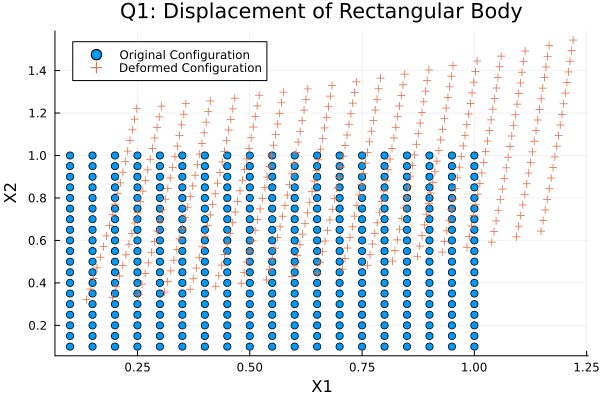
\includegraphics[width=0.5\linewidth]{media/Displacement_of_Rectangular_Body.png}
        \caption{Displacement of Rectangular Body}
        \label{fig:solution1}
    \end{figure}
    
\end{solution}  

\question  With respect to a two-dimensional rectangular cartesian coordinates system with orthonormal base vectors $(e_{1},e_{2})$, let the rectangular coordinates of a point be denoted by $(X_{1},X_{2})$. Consider a two-dimensional annular body $\mathcal{B}$ which occupies the region:
\[ \mathcal{B}=\{(X_{1},X_{2})|1<\sqrt{X_{1}^{2}+X_{2}^{2}}<2\} \].

Because of the annual nature of the body consider a polar coordinates system in which the coordinates of points are expressed in terms $(R, \theta)$, which are related to the rectangular coordinates $(X_{1},X_{2})$ by:
\[ R=\sqrt{X_{1}^{2}+X_{2}^{2}} and \theta=\tan^{-1}(X_{2}/X_{1}) \]

Further, the orthonormal base vectors $(e_{r},e_{\theta})$ of the polar coordinate system are related to $(e_{1},e_{2})$ by:
$$e_{r}=\cos \theta e_{1}+\sin \theta e_{2}, e_{\theta}=-\sin \theta e_{1}+\cos \theta e_{2}$$

Draw the deformed configuration of the annular body associated with the following deformation using Julia:
\[u_{r}=u\cdot e_{r}=0.4(R-1)^{2}\cos 3\theta  \]
\[ u_{\theta}=u\cdot e_{\theta}=0.4(R-1)^{3} \]

**Hint:**
First set up some characteristic lines on the body in terms of their $(R, \theta)$ coordinates. Compute the $(X_{1},X_{2})$ coordinates from $$X_{1}=R \cos \theta, X_{2}=R \sin \theta$$.
For each point compute its displacement and add it to the original position by noting $x_{i}=e_{i}\cdot(X+u)=e_{i}\cdot(X+u_{r}e_{r}+u_{\theta}e_{\theta})$.

\begin{solution}
    \textbf{Solution: 2}
    \begin{minted}{julia}
        using Plots
        
        # 1. Define the annular domain using Polar Coordinates
        R_range = 1.0:0.1:2.0
        Theta_range = 0:0.01:2*pi
        
        X1_orig, X2_orig = Float64[], Float64[]
        x1_new, x2_new = Float64[], Float64[]
        
        for r in R_range
            for theta in Theta_range
                # Convert Polar to Cartesian for Original Points [cite: 33]
                X1 = r * cos(theta)
                X2 = r * sin(theta)
                
                push!(X1_orig, X1)
                push!(X2_orig, X2)
        
                # Calculate Displacements in Polar Basis [cite: 29]
                u_r = 0.4 * (r - 1)^2 * cos(3 * theta)
                u_theta = 0.4 * (r - 1)^3
        
                # Transformation to Cartesian Basis
                # u1 = u_r * cos(theta) - u_theta * sin(theta)
                # u2 = u_r * sin(theta) + u_theta * cos(theta)
                # Derived from basis vector relations [cite: 25, 34]
                
                u1 = u_r * cos(theta) - u_theta * sin(theta)
                u2 = u_r * sin(theta) + u_theta * cos(theta)
        
                # Add displacement to original Cartesian coords
                push!(x1_new, X1 + u1)
                push!(x2_new, X2 + u2)
            end
        end
        
        # 3. Plotting
        scatter(X1_orig, X2_orig, label="Original", aspect_ratio=:equal, markersize=2)
        scatter!(x1_new, x2_new, label="Deformed", markersize=2)
        title!("Q2: Annular Body Deformation")
        
        savefig("Annular_Body_Deformation.png")   # save the figure
    \end{minted}

    \begin{figure}[H]
        \centering
        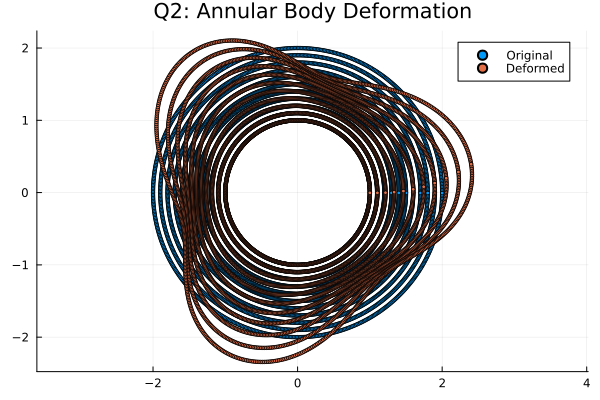
\includegraphics[width=0.5\linewidth]{media/Annular_Body_Deformation.png}
        \caption{Annular Body Deformation}
        \label{fig:solution2}
    \end{figure}
    
\end{solution}

\question Given the two-dimensional body
\[\mathcal{B}=\{(X_{1},X_{2})|0.1<X_{1}<1, 0.1<X_{2}<1\}\],

and the displacement field
\[u_{r}=u\cdot e_{r}=0.2 \exp X_{1},  
u_{\theta}=u\cdot e_{\theta}=0.2 \ln(1+X_{1}+X_{2})\].

Plot the displaced shape of the body using Julia.

\begin{solution}
    \textbf{Solution: 3}
    
    \begin{minted}{julia}
        using Plots
        
        x1_range = 0.1:0.05:1.0
        x2_range = 0.1:0.05:1.0
        
        X1_orig, X2_orig = Float64[], Float64[]
        x1_new, x2_new = Float64[], Float64[]
        
        for X1 in x1_range
            for X2 in x2_range
                push!(X1_orig, X1)
                push!(X2_orig, X2)
        
                # Calculate local polar parameters for basis transformation [cite: 23]
                R = sqrt(X1^2 + X2^2)
                theta = atan(X2, X1)
        
                # Calculate displacements (given values) [cite: 38, 40]
                u_r_val = 0.2 * exp(X1)
                u_theta_val = 0.2 * log(1 + X1 + X2)
        
                # Convert to Cartesian components u1, u2 using local theta
                # u = u_r * e_r + u_theta * e_theta
                u1 = u_r_val * cos(theta) - u_theta_val * sin(theta)
                u2 = u_r_val * sin(theta) + u_theta_val * cos(theta)
        
                push!(x1_new, X1 + u1)
                push!(x2_new, X2 + u2)
            end
        end
        
        scatter(X1_orig, X2_orig, label="Original", legend=:topleft)
        scatter!(x1_new, x2_new, label="Deformed")
        title!("Q3: Mixed Basis Deformation")
        
        savefig("Mixed_Basis_Deformation.png")   # save the figure
    \end{minted}
    
    \begin{figure}[H]
        \centering
        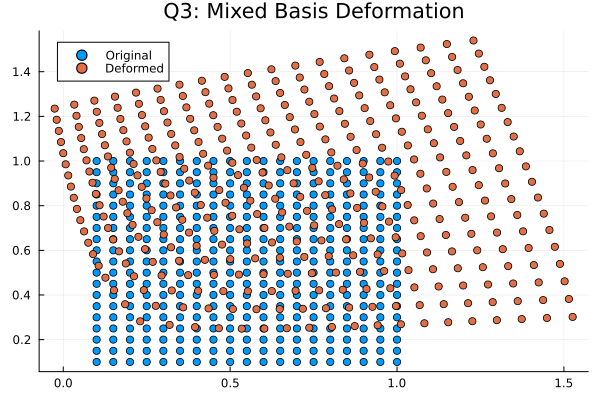
\includegraphics[width=0.5\linewidth]{media/Mixed_Basis_Deformation.png}
        \caption{Mixed Basis Deformation}
        \label{fig:solution3}
    \end{figure}
\end{solution}

\question  Find out the stress distribution by modeling the given rectangular plate of 2 mm thick with a circular hole. The dimensions of the steel plate and hole are shown in Figure 1. The section is made up of steel having a value of 210 GPa for Young's modulus and a value of 0.3 for Poisson's ratio.\\

\begin{figure}[H]
    \centering
    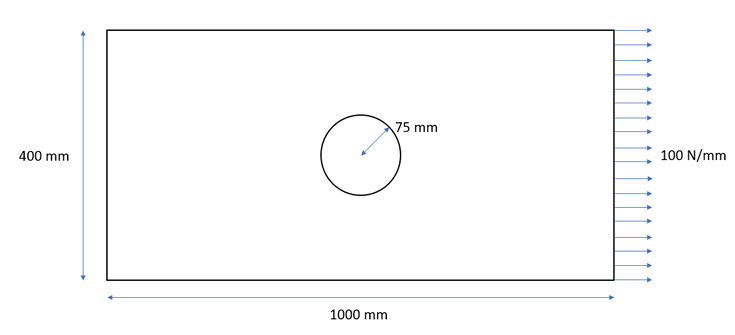
\includegraphics[width=0.5\linewidth]{media/figure1.png}
    \caption{Caption}
    \label{fig:placeholder}
\end{figure} 

\noindent(a) Provide the steps for finite element meshing both in Julia and Abaqus.  \\
(b) Mention the governing PDEs that are required to solve for the stress distribution.  \\
(c) Provide a comparison between the results obtained from Gridap in Julia and Abaqus.

\begin{solution}
    \textbf{Solution: 4}
    (a) Steps for finite element meshing using Julia. 
    \sloppy
    \begin{minted}{julia}
        import Gmsh: gmsh
        
        # Initializing Gmsh
        gmsh.initialize()
        
        gmsh.model.add("PlateHole_Q4")
        
        # --- Parameters (Converted to Meters to match your L=1 scale) ---
        L = 1.0      # 1000 mm
        H = 0.4      # 400 mm
        R = 0.075    # Radius 75 mm
        Xc = 0.5     # Center X (500 mm)
        Yc = 0.2     # Center Y (200 mm)
        
        # Mesh sizes
        h_coarse = 0.008  # Coarse mesh for far boundaries
        h_fine   = 0.005 # Fine mesh for the hole (CRITICAL for stress concentration)
        
        # --- 1. Define the Outer Rectangle ---
        p1 = gmsh.model.geo.addPoint(0, 0, 0, h_coarse)
        p2 = gmsh.model.geo.addPoint(L, 0, 0, h_coarse)
        p3 = gmsh.model.geo.addPoint(L, H, 0, h_coarse)
        p4 = gmsh.model.geo.addPoint(0, H, 0, h_coarse)
        
        l1 = gmsh.model.geo.addLine(p1, p2)
        l2 = gmsh.model.geo.addLine(p2, p3)
        l3 = gmsh.model.geo.addLine(p3, p4)
        l4 = gmsh.model.geo.addLine(p4, p1)
        
        # Outer Loop
        cl_rect = gmsh.model.geo.addCurveLoop([l1, l2, l3, l4])
        
        # --- 2. Define the Inner Circle ---
        # We create 5 points: Center + 4 points on the circumference (Top, Right, Bottom, Left)
        # This method (Circle Arcs) is more robust for meshing than a single full circle.
        
        pc = gmsh.model.geo.addPoint(Xc, Yc, 0, h_fine) # Center
        p_r = gmsh.model.geo.addPoint(Xc + R, Yc, 0, h_fine)
        p_t = gmsh.model.geo.addPoint(Xc, Yc + R, 0, h_fine)
        p_l = gmsh.model.geo.addPoint(Xc - R, Yc, 0, h_fine)
        p_b = gmsh.model.geo.addPoint(Xc, Yc - R, 0, h_fine)
        
        # Create 4 arcs to form the circle
        c1 = gmsh.model.geo.addCircleArc(p_r, pc, p_t)
        c2 = gmsh.model.geo.addCircleArc(p_t, pc, p_l)
        c3 = gmsh.model.geo.addCircleArc(p_l, pc, p_b)
        c4 = gmsh.model.geo.addCircleArc(p_b, pc, p_r)
        
        # Inner Loop
        cl_hole = gmsh.model.geo.addCurveLoop([c1, c2, c3, c4])
        
        # --- 3. Create Surface with Hole ---
        # The first loop is the boundary, subsequent loops are holes
        s = gmsh.model.geo.addPlaneSurface([cl_rect, cl_hole])
        
        # --- 4. Physical Groups (Boundary Conditions) ---
        # Domain
        gmsh.model.addPhysicalGroup(2, [s], 1, "Plate")
        
        # Boundaries
        gmsh.model.addPhysicalGroup(1, [l4], 2, "FixedLeft")  # Left Edge
        gmsh.model.addPhysicalGroup(1, [l2], 3, "LoadRight")  # Right Edge
        gmsh.model.addPhysicalGroup(1, [c1, c2, c3, c4], 4, "HoleEdge") # Hole boundary
        
        # Synchronize and Mesh
        gmsh.model.geo.synchronize()
        gmsh.model.mesh.generate(2)
        
        # Write mesh to file
        gmsh.write("PlateHole_Q4.msh")
        
        # Launch GUI to see the result
        gmsh.fltk.run()
        gmsh.finalize()
    \end{minted}
    
    \begin{figure}[H]
        \centering
        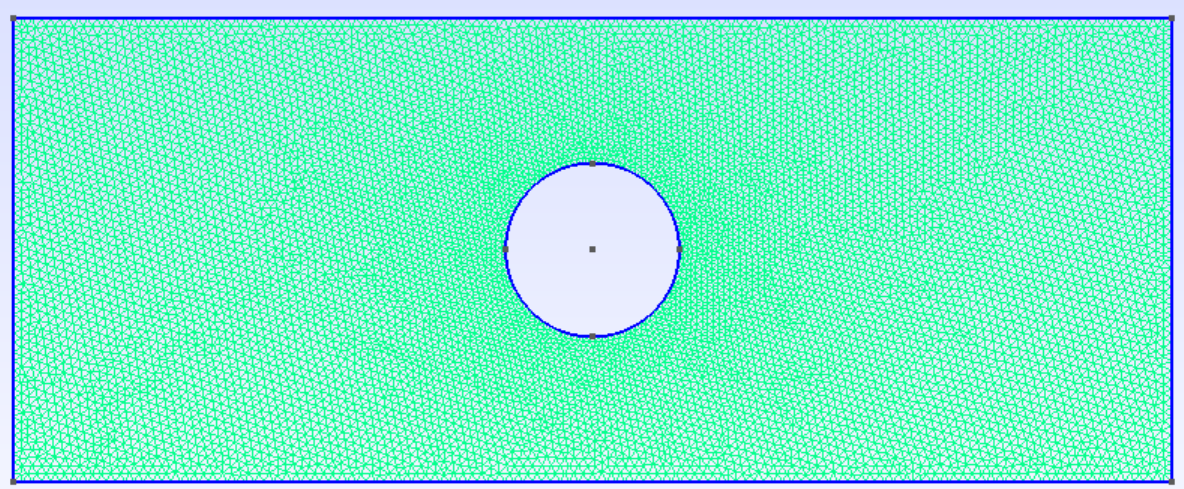
\includegraphics[width=0.5\linewidth]{media/meshing_Q4.png}
        \caption{ Finite element meshing using Julia. }
        \label{fig:Julia}
    \end{figure}
    
    4(a) Steps for finite element meshing using Abaqus. 
    \begin{enumerate}
        \item Create a 2D deformable part
        \begin{itemize}
            \item Start Abaqus/CAE → go to the Part module.
            \item Create a new part:
            \begin{itemize}
                \item Name: PlateHole$\_$Q4.
                \item Modeling space: 2D planar.
                \item Type: Deformable.
                \item Base feature: Shell (plane stress) or Planar.
                \item  Approximate size: slightly larger than 2000 mm.
            \end{itemize}
        \end{itemize}
        \item Sketch the plate geometry
        \begin{itemize}
            \item In the sketcher, draw a rectangle representing the plate:
            \begin{itemize}
                \item One corner at (0,0).
                \item Opposite corner at (1000,400) mm (length × height).
            \end{itemize}
            \item In the same sketch, create a circle with:
            \begin{itemize}
                \item Center at (500,200) mm and Radius = 75 mm.
            \end{itemize}
            \item Finish the sketch to form the final 2D plate-with-hole geometry.
        \end{itemize}
        \item Define material and section (for completeness)
        \begin{itemize}
            \item Go to the Property module.
            \item Create a material:
            \begin{itemize}
                \item Name: Steel.
                \item Elastic properties: Young’s modulus E=210 GPa Poisson’s ratio $\nu$ =0.3.
            \end{itemize}
            \item Create a solid/plane stress section: Thickness = 2 mm.
            \item Assign this section to the entire plate part.
        \end{itemize}
        \item Create assembly
        \begin{itemize}
            \item Move to the Assembly module.
            \item Create a dependent instance of the part (Create Instance).
        \end{itemize}
        \item Choose element type
        \begin{itemize}
            \item Go to the Mesh module.
            \item Assign element type:
            \begin{itemize}
                \item Element family: plane stress (e.g., CPS4/CPS4R).
                \item Suitable for 2D stress analysis of thin plate.
            \end{itemize}
        \end{itemize}
        \item Seed the edges (global and local refinement)
        \begin{itemize}
            \item Apply a global seed size (coarse mesh) for the plate
            \item Apply a smaller seed size on the hole boundary
        \end{itemize}
        \item Generate the mesh
        \begin{itemize}
            \item With seeding done, Abaqus will generate the 2D finite element mesh for the plate with a hole
        \end{itemize}
    \end{enumerate}

    \begin{figure}[H]
        \centering
        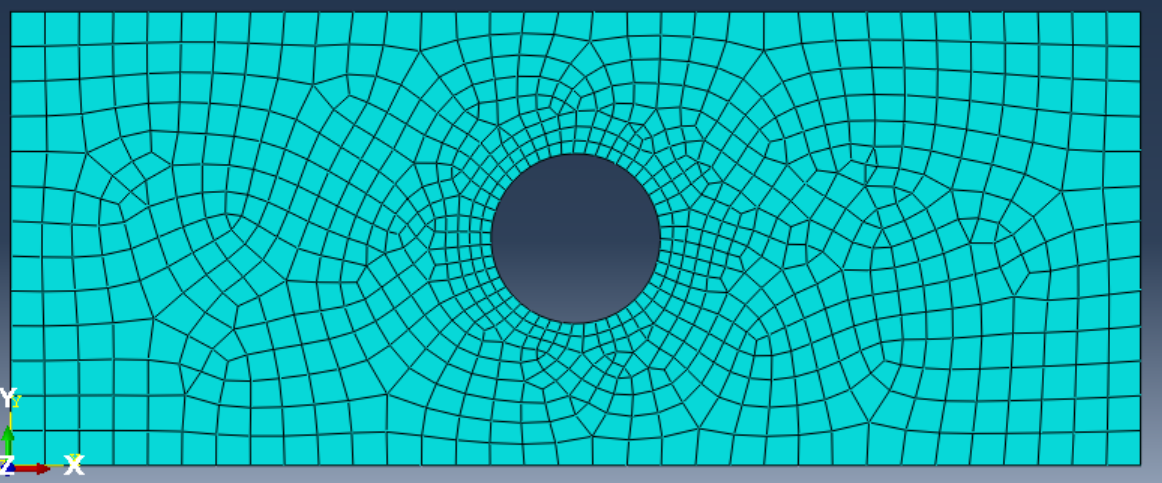
\includegraphics[width=0.5\linewidth]{media/Meshing_Q4_Abaqus.png}
        \caption{ Finite element meshing using Abaqus }
        \label{fig:Abaqus}
    \end{figure}

    \textbf{Solution: 4}
    (b)  Stress distribution. 
    \sloppy
    \begin{minted}{julia}
        using Gridap
        using GridapGmsh
        
        # 1. Read the Mesh
        model = GmshDiscreteModel("PlateHole_Q4.msh")
        
        # 2. Material Parameters (Steel)
        const E = 210000.0  # MPa
        const ν = 0.3       # Poisson's ratio
        const thickness = 2.0 # mm
        
        # Lamé parameters for Plane Stress
        const E = 210000.0                              # N/mm^2
        const ν = 0.3                                   # Poissons Ratio
        
        const μ = E/(2*(1+ν))
        const λ = (E * ν) / ((1 + ν) * (1 - 2 * ν))
        const λ_ps = (2 * λ * μ) / (λ + 2 * μ)          # Plane stress correction
        
        g = VectorValue(100.0, 0.0)                # Force
        
        σ(ε) = λ_ps*tr(ε)*one(ε) + 2*μ*ε
        
        # 3. Define FE Spaces
        order = 1
        
        reffe = ReferenceFE(lagrangian,VectorValue{2,Float64},order)
        V0 = TestFESpace(model,reffe;
            conformity=:H1,
            dirichlet_tags=["FixedLeft"],
            dirichlet_masks=[(true,true)])
          
        g1 = VectorValue(0.0,0.0)
        U = TrialFESpace(V0,[g1])
        
        # 4. Numerical Integration
        degree = 2*order
        Ω = Triangulation(model)
        dΩ = Measure(Ω,degree)
        Γ_load  = BoundaryTriangulation(model, tags = "LoadRight")
        dΓ_N = Measure(Γ_load,degree)
        
        # 5. Define Weak Form
        
        # Internal Work (Stiffness)
        a(u,v) = ∫( ε(v) ⊙ (σ∘ε(u)) )*dΩ 
        
        # External Work (Load)
        l(v) = ∫(v⋅g)*dΓ_N
        
        # 6. Solve
        op = AffineFEOperator(a,l,U,V0)
        uh = solve(op)
        
        # 7. Post-Process
        writevtk(Ω,"results_Q4",
            cellfields=[
                "Displacement"=>uh,
                "Strain"=>ε(uh),
                "Stress"=>σ∘ε(uh)]
                )

    \end{minted}

    4(c) Comparison between the results obtained from Gridap in Julia and Abaqus.

\begin{figure}[H]
    \centering
    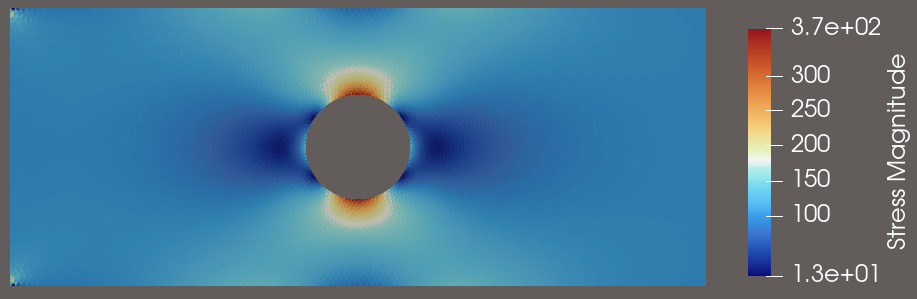
\includegraphics[width=0.5\linewidth]{media/ResultQ4julia.png}
    \caption{Stress distribution using Julia.}
    \label{fig:ResultQ4julia}
\end{figure}

\begin{figure}[H]
    \centering
    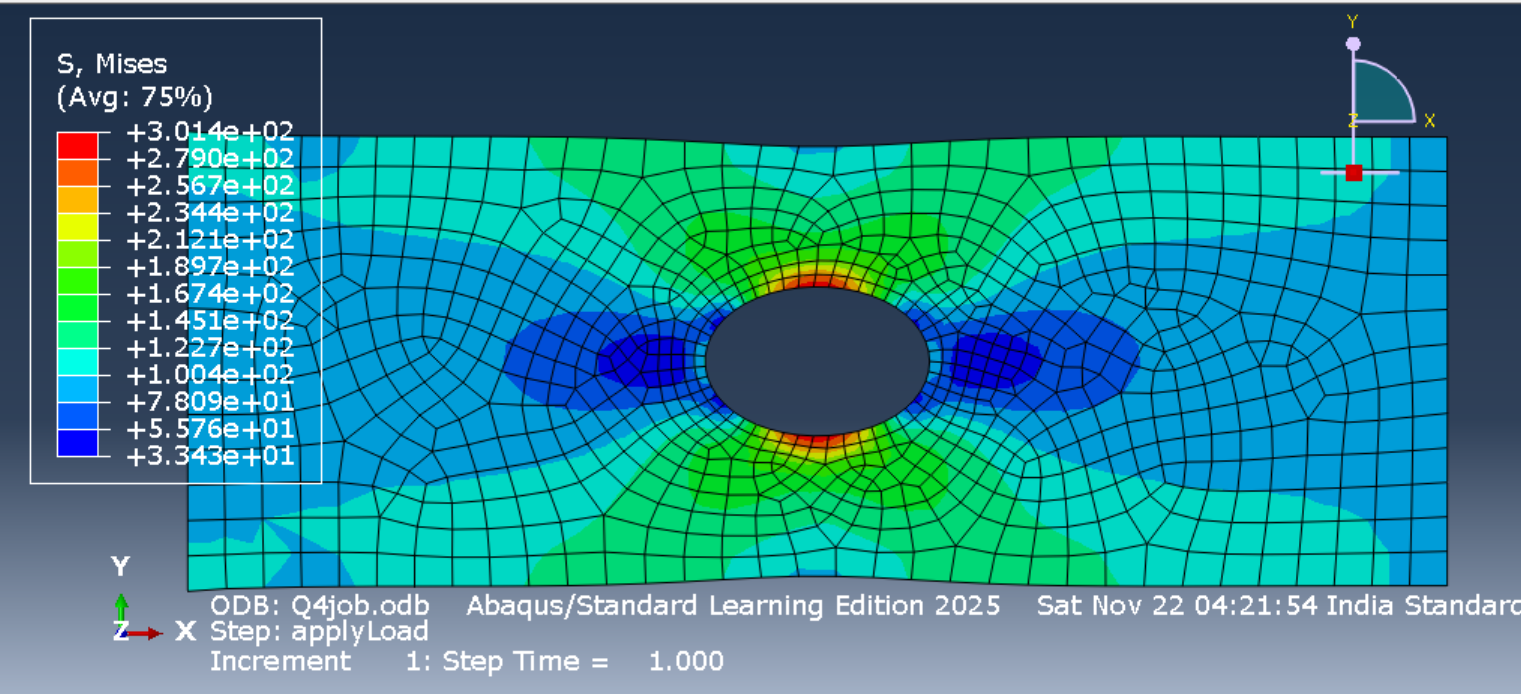
\includegraphics[width=0.5\linewidth]{media/resultQ4Abaqus.png}
    \caption{Stress distribution using Julia.}
    \label{fig:resultQ4Abaqus}
\end{figure}

\end{solution}


\question Find out the stress distribution of the cantilever beam of 1000 mm in length and has a $250 \text{ mm} \times 200 \text{ mm}$ rectangular cross-section under the point load of 1000 N at the free end as shown in Figure 2. The section is made up of a concrete having a value of 25000 N/mm² for Young's modulus and a value of 0.2 for Poisson's ratio in the respective fields.\\

\begin{figure}[H]
    \centering
    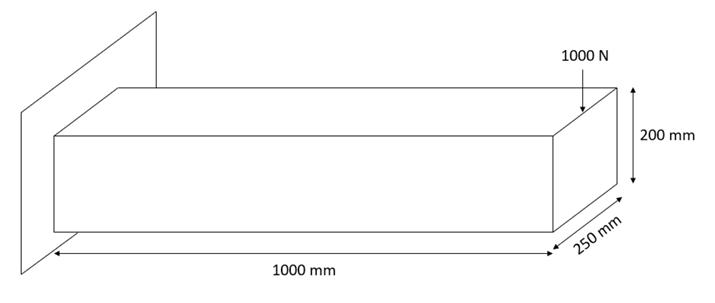
\includegraphics[width=0.5\linewidth]{media/figure2.png}
    \caption{Caption}
    \label{fig:placeholder}
\end{figure}

\noindent (a) Provide the steps for finite element meshing both in Julia and Abaqus.  \\
(b) Mention the governing PDEs that are required to solve for the stress distribution.  \\
(c) Provide a comparison between the results obtained from Gridap in Julia and Abaqus.

\begin{solution}
    \textbf{Solution: 5}
    (a) Steps for finite element meshing using Julia. 
    \sloppy
    \begin{minted}{julia}
        using Gmsh: gmsh
        
        # Dimensions
        L = 1000.0   # x-direction (length)
        W = 250.0    # y-direction (width)
        H = 200.0    # z-direction (height)
        h = 10.0     # mesh size
        
        gmsh.initialize()
        gmsh.model.add("Cantilever_Q5")
        
        # --- Create the 8 corner points of the box ---
        p1 = gmsh.model.geo.addPoint(0, 0, 0, h)
        p2 = gmsh.model.geo.addPoint(L, 0, 0, h)
        p3 = gmsh.model.geo.addPoint(L, W, 0, h)
        p4 = gmsh.model.geo.addPoint(0, W, 0, h)
        
        p5 = gmsh.model.geo.addPoint(0, 0, H, h)
        p6 = gmsh.model.geo.addPoint(L, 0, H, h)
        p7 = gmsh.model.geo.addPoint(L, W, H, h)
        p8 = gmsh.model.geo.addPoint(0, W, H, h)
        
        # --- Create lines for bottom face ---
        l1 = gmsh.model.geo.addLine(p1, p2)
        l2 = gmsh.model.geo.addLine(p2, p3)
        l3 = gmsh.model.geo.addLine(p3, p4)
        l4 = gmsh.model.geo.addLine(p4, p1)
        
        # --- Create lines for top face ---
        l5 = gmsh.model.geo.addLine(p5, p6)
        l6 = gmsh.model.geo.addLine(p6, p7)
        l7 = gmsh.model.geo.addLine(p7, p8)
        l8 = gmsh.model.geo.addLine(p8, p5)
        
        # --- Side edges ---
        l9  = gmsh.model.geo.addLine(p1, p5)
        l10 = gmsh.model.geo.addLine(p2, p6)
        l11 = gmsh.model.geo.addLine(p3, p7)
        l12 = gmsh.model.geo.addLine(p4, p8)
        
        # ---- Create surfaces (6 faces of the box) ----
        
        # Bottom rectangle
        cl1 = gmsh.model.geo.addCurveLoop([l1, l2, l3, l4])
        s1  = gmsh.model.geo.addPlaneSurface([cl1])
        
        # Top rectangle
        cl2 = gmsh.model.geo.addCurveLoop([l5, l6, l7, l8])
        s2  = gmsh.model.geo.addPlaneSurface([cl2])
        
        # Side faces
        cl3 = gmsh.model.geo.addCurveLoop([l1, l10, -l5, -l9])
        s3  = gmsh.model.geo.addPlaneSurface([cl3])
        
        cl4 = gmsh.model.geo.addCurveLoop([l2, l11, -l6, -l10])
        s4  = gmsh.model.geo.addPlaneSurface([cl4])
        
        cl5 = gmsh.model.geo.addCurveLoop([l3, l12, -l7, -l11])
        s5  = gmsh.model.geo.addPlaneSurface([cl5])
        
        cl6 = gmsh.model.geo.addCurveLoop([l4, l9, -l8, -l12])
        s6  = gmsh.model.geo.addPlaneSurface([cl6])
        
        # ---- Create 3D volume ----
        sl = gmsh.model.geo.addSurfaceLoop([s1, s2, s3, s4, s5, s6])
        vol = gmsh.model.geo.addVolume([sl])
        
        gmsh.model.geo.synchronize()
        
        # ---- Physical groups ----
        
        # 3D domain
        gmsh.model.addPhysicalGroup(3, [vol], 10, "Domain")
        
        # Fixed End (x = 0 → face s6)
        gmsh.model.addPhysicalGroup(2, [s6], 2)
        gmsh.model.setPhysicalName(2, 2, "FixedEnd")
        
        # Load End (x = L → face s4)
        gmsh.model.addPhysicalGroup(2, [s4], 3)
        gmsh.model.setPhysicalName(2, 3, "LoadFace")
        
        # ---- Mesh ----
        gmsh.model.mesh.generate(3)
        
        # Export mesh
        gmsh.write("Cantilever_Q5.msh")
        
        # View mesh
        gmsh.fltk.run()
        gmsh.finalize()
    \end{minted}

    \begin{figure}[H]
        \centering
        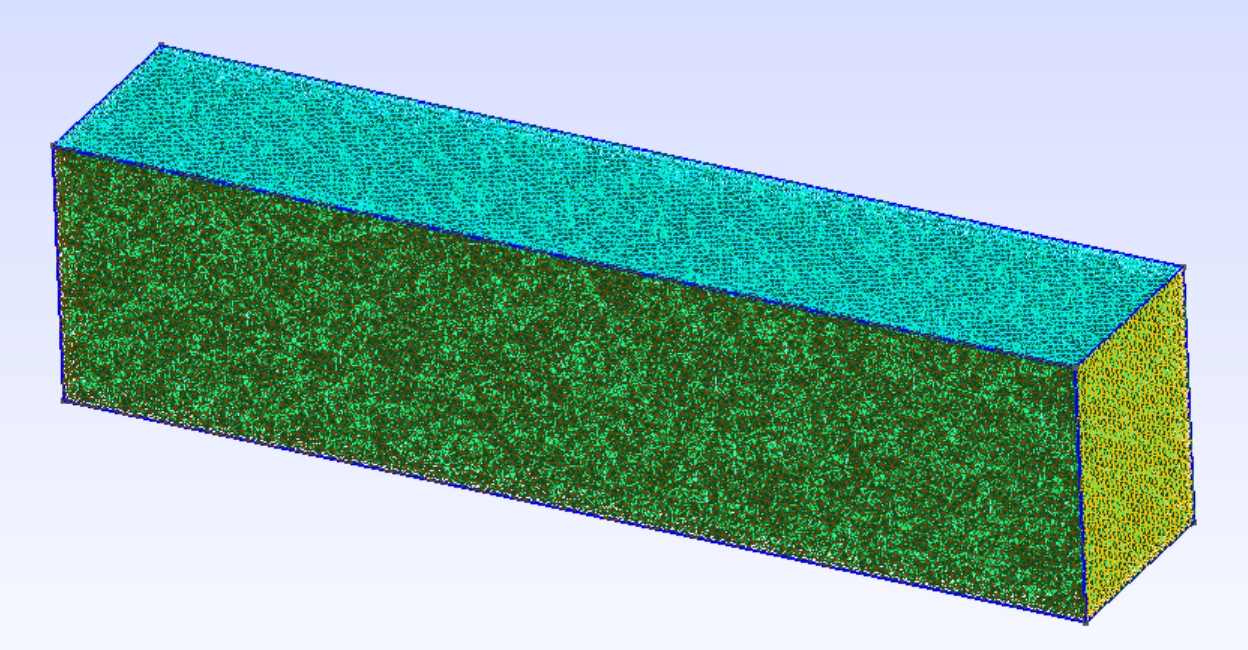
\includegraphics[width=0.5\linewidth]{media/meshing_Q5.png}
        \caption{Finite element meshing using Julia.}
        \label{fig:Julia-2}
    \end{figure}

5(a)\label{prob:{5a}} Steps for finite element meshing using Abaqus. 
    \begin{enumerate}
        \item Create a 3D deformable solid part
        \begin{itemize}
            \item Start Abaqus/CAE → go to the Part module.
            \item Create a new part:
            \begin{itemize}
                \item Name: Cantilever$\_$Q5.
                \item Modeling space: 3D.
                \item Type: Deformable.
                \item Base feature: Solid, Extrusion (or Solid).
                \item  Approximate size: slightly larger than 2000 mm.
            \end{itemize}
        \end{itemize}
        \item Sketch the cross-section and define the beam length
        \begin{itemize}
            \item In the sketcher, draw a rectangle representing the cross-section:
            \begin{itemize}
                \item Width = 250 mm, Height = 200 mm.
                \item Finish the sketch.
                \item When prompted for extrusion: Extrusion length = 1000 mm (this is the beam length).
            \end{itemize}
        \end{itemize}
        \item Define material and solid section
        \begin{itemize}
            \item Go to the Property module.
            \item Create a material:
            \begin{itemize}
                \item Name: Concrete.
                \item Elastic properties: Young’s modulus E=25000 N/mm2, Poisson’s ratio $\nu$ =0.2.
            \end{itemize}
            \item Create a solid section (e.g. “BeamSection”) and assign the material Concrete.
            \item Assign this section to the entire beam part.
        \end{itemize}
        \item Create assembly
        \begin{itemize}
            \item Move to the Assembly module.
            \item Create a dependent instance of the part (Create Instance).
        \end{itemize}
        \item Choose element type and seed the part.
        \begin{itemize}
            \item Go to the Mesh module.
            \item Assign element type:
            \begin{itemize}
                \item Choose 3D stress elements, e.g. C3D8 or C3D8R (8-node linear brick, reduced integration).
                \item Confirm and apply to the solid region.
                \item Choose a suitable global seed size along the beam length and across the cross-section.
            \end{itemize}
        \end{itemize}
        \item Generate the mesh
        \begin{itemize}
            \item With seeding done, Abaqus generates the 3D finite element mesh for the cantilever beam.
        \end{itemize}
    \end{enumerate}


    \begin{figure}[H]
        \centering
        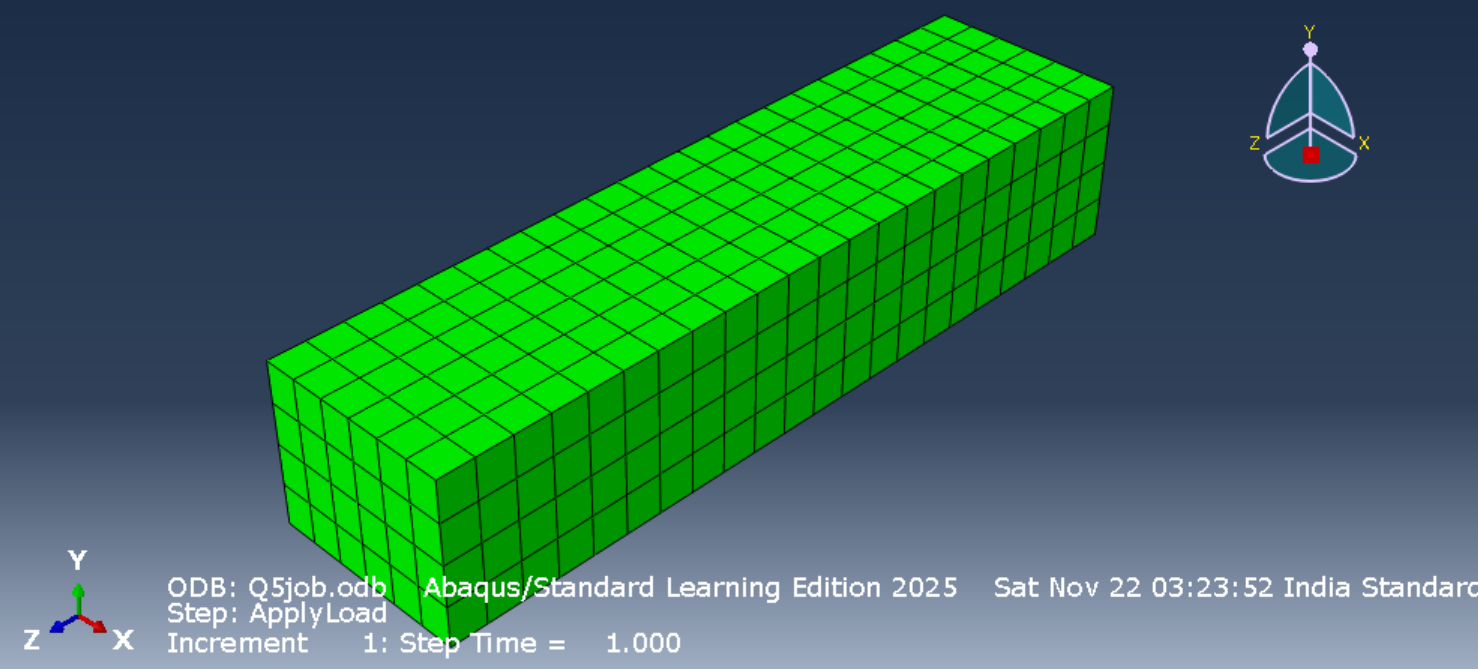
\includegraphics[width=0.5\linewidth]{media/meshing_Q5_Abaqus.png}
        \caption{Finite element meshing using Abaqus.}
        \label{fig:Abaqus-2}
    \end{figure}


    \textbf{Solution: 5}
    (b)  Stress distribution. 
    \sloppy
    \begin{minted}{julia}
        using Gridap
        using GridapGmsh
        # 1. Read the Mesh
        model = GmshDiscreteModel("Cantilever_Q5.msh")
        
        # 2. Material Parameters (Steel)
        const E = 25000.0  # MPa
        const ν = 0.2       # Poisson's ratio
        
        # Lamé parameters for Plane Stress
        
        g = VectorValue(0.0,0.0,-1000.0/(250*200)) ## force
        
        const λ = (E*ν)/((1+ν)*(1-2*ν))
        const μ = E/(2*(1+ν))
        σ(ε) = λ*tr(ε)*one(ε) + 2*μ*ε
        
        # 3. Define FE Spaces
        order = 1
        
        reffe = ReferenceFE(lagrangian,VectorValue{3,Float64},order)
        V0 = TestFESpace(model,reffe;
            conformity=:H1,
            dirichlet_tags=["FixedEnd"],
            dirichlet_masks=[(true,true,true)])
          
        g1 = VectorValue(0.0,0.0,0.0)
        U = TrialFESpace(V0,[g1])
        
        # 4. Numerical Integration
        degree = 2*order
        Ω = Triangulation(model)
        dΩ = Measure(Ω,degree)
        Γ_load  = BoundaryTriangulation(model, tags = "LoadFace")
        dΓ_N = Measure(Γ_load,degree)
        
        # Weak from
        
        # Internal work (Stiffness component)
        a(u,v) = ∫( ε(v) ⊙ (σ∘ε(u)) )*dΩ 
        
        # External Work
        l(v) = ∫(v⋅g)*dΓ_N
        
        # Solve
        op = AffineFEOperator(a,l,U,V0)
        uh = solve(op)
        
        # 7. Post-Process
        writevtk(Ω,"results_Q5",
            cellfields=[
                "Displacement"=>uh,
                "Strain"=>ε(uh),
                "Stress"=>σ∘ε(uh)]
                )
        
    \end{minted}

     5(c) Comparison between the results obtained from Gridap in Julia and Abaqus.

     \begin{figure}[H]
         \centering
         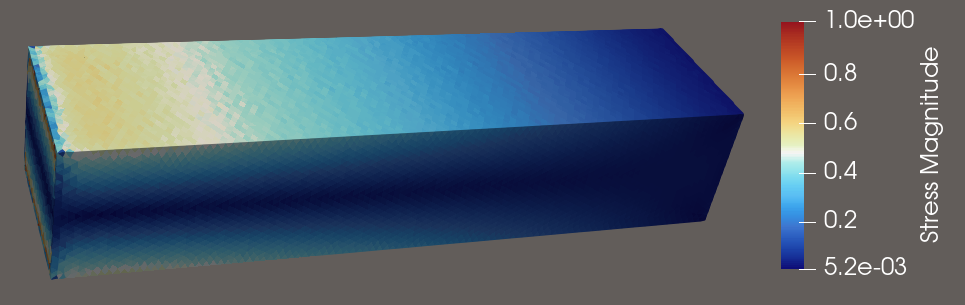
\includegraphics[width=0.5\linewidth]{media/ResultQ5julia.png}
         \caption{Stress distribution using julia}
         \label{fig:ResultQ5julia}
     \end{figure}

     \begin{figure}[H]
         \centering
         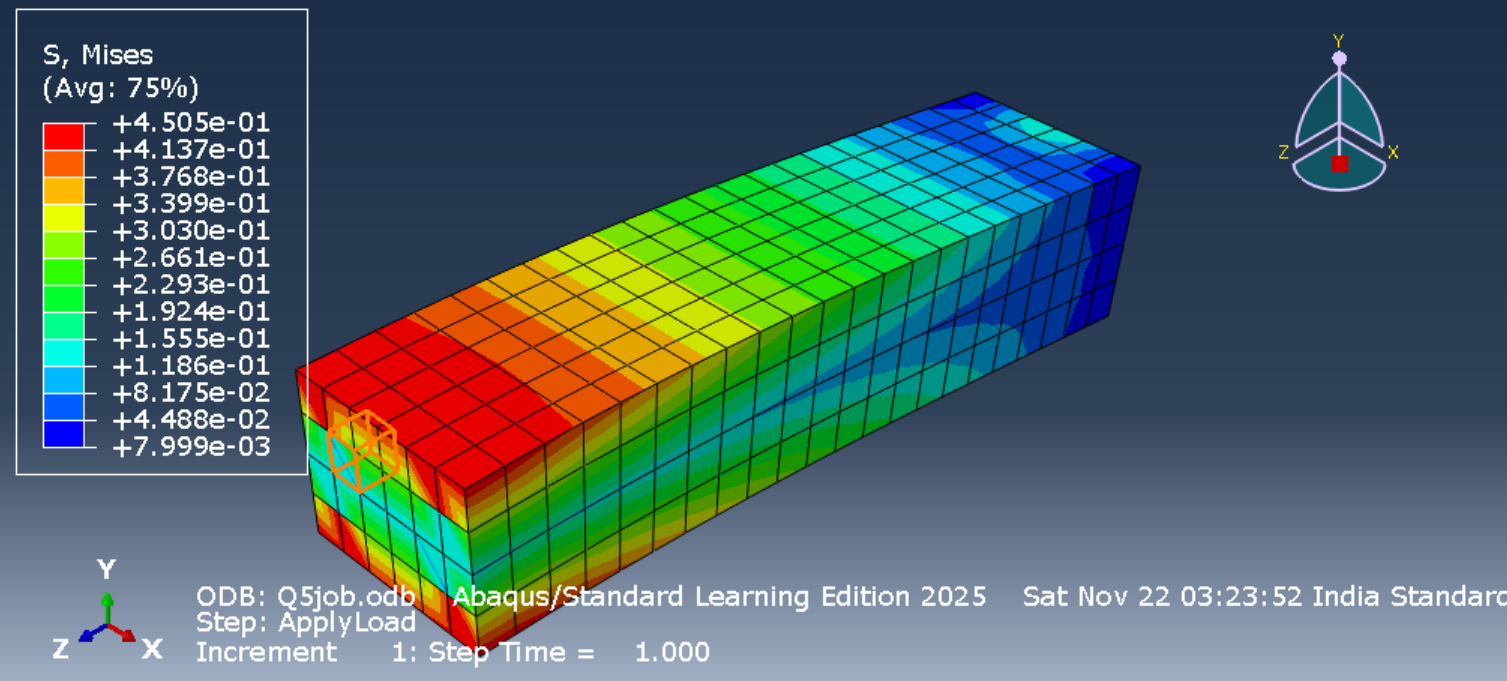
\includegraphics[width=0.5\linewidth]{media/ResultQ5Abaqus.png}
         \caption{Stress distribution using Abaqus}
         \label{fig:ResultQ5Abaqus}
     \end{figure}
     
\end{solution}

\question  Find out the stress distribution of the cantilever beam of 1000 mm in length and has a $250 \text{ mm} \times 200 \text{ mm}$ rectangular cross-section under the uniform distributed load of 1000 N/mm² applied on the top surface as shown in Figure 3. The section is made up of a concrete having a value of 25000 N/mm² for Young's modulus and a value of 0.2 for Poisson's ratio in the respective fields.

\begin{figure}[H]
    \centering
    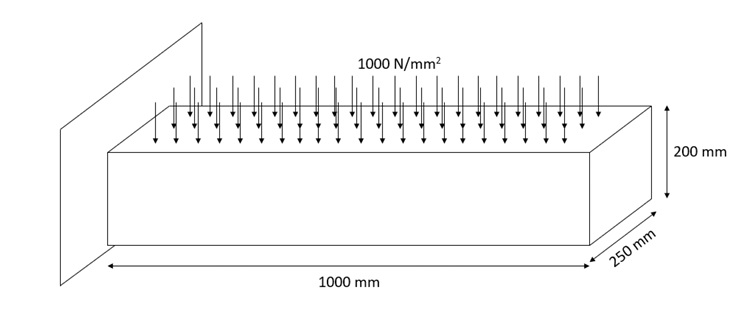
\includegraphics[width=0.5\linewidth]{media/figure3.png}
    \caption{Caption}
    \label{fig:placeholder}
\end{figure}

\noindent (a) Provide the steps for finite element meshing both in Julia and Abaqus. \\ 
(b) Mention the governing PDEs that are required to solve for the stress distribution.  \\
(c) Provide a comparison between the results obtained from Gridap in Julia and Abaqus.

\begin{solution}
    \textbf{Solution: 6}
    (a) Steps for finite element meshing using Julia. 
    \sloppy
    \begin{minted}{julia}
        using Gmsh: gmsh

        # Dimensions
        L = 1000.0   # x-direction (length)
        W = 250.0    # y-direction (width)
        H = 200.0    # z-direction (height)
        h = 10.0     # mesh size
        
        gmsh.initialize()
        gmsh.model.add("Cantilever_Q6")
        
        # --- Create the 8 corner points of the box ---
        p1 = gmsh.model.geo.addPoint(0, 0, 0, h)
        p2 = gmsh.model.geo.addPoint(L, 0, 0, h)
        p3 = gmsh.model.geo.addPoint(L, W, 0, h)
        p4 = gmsh.model.geo.addPoint(0, W, 0, h)
        
        p5 = gmsh.model.geo.addPoint(0, 0, H, h)
        p6 = gmsh.model.geo.addPoint(L, 0, H, h)
        p7 = gmsh.model.geo.addPoint(L, W, H, h)
        p8 = gmsh.model.geo.addPoint(0, W, H, h)
        
        # --- Create lines for bottom face ---
        l1 = gmsh.model.geo.addLine(p1, p2)
        l2 = gmsh.model.geo.addLine(p2, p3)
        l3 = gmsh.model.geo.addLine(p3, p4)
        l4 = gmsh.model.geo.addLine(p4, p1)
        
        # --- Create lines for top face ---
        l5 = gmsh.model.geo.addLine(p5, p6)
        l6 = gmsh.model.geo.addLine(p6, p7)
        l7 = gmsh.model.geo.addLine(p7, p8)
        l8 = gmsh.model.geo.addLine(p8, p5)
        
        # --- Side edges ---
        l9  = gmsh.model.geo.addLine(p1, p5)
        l10 = gmsh.model.geo.addLine(p2, p6)
        l11 = gmsh.model.geo.addLine(p3, p7)
        l12 = gmsh.model.geo.addLine(p4, p8)
        
        # ---- Create surfaces (6 faces of the box) ----
        
        # Bottom rectangle
        cl1 = gmsh.model.geo.addCurveLoop([l1, l2, l3, l4])
        s1  = gmsh.model.geo.addPlaneSurface([cl1])
        
        # Top rectangle
        cl2 = gmsh.model.geo.addCurveLoop([l5, l6, l7, l8])
        s2  = gmsh.model.geo.addPlaneSurface([cl2])
        
        # Side faces
        cl3 = gmsh.model.geo.addCurveLoop([l1, l10, -l5, -l9])
        s3  = gmsh.model.geo.addPlaneSurface([cl3])
        
        cl4 = gmsh.model.geo.addCurveLoop([l2, l11, -l6, -l10])
        s4  = gmsh.model.geo.addPlaneSurface([cl4])
        
        cl5 = gmsh.model.geo.addCurveLoop([l3, l12, -l7, -l11])
        s5  = gmsh.model.geo.addPlaneSurface([cl5])
        
        cl6 = gmsh.model.geo.addCurveLoop([l4, l9, -l8, -l12])
        s6  = gmsh.model.geo.addPlaneSurface([cl6])
        
        # ---- Create 3D volume ----
        sl = gmsh.model.geo.addSurfaceLoop([s1, s2, s3, s4, s5, s6])
        vol = gmsh.model.geo.addVolume([sl])
        
        gmsh.model.geo.synchronize()
        
        # ---- Physical groups ----
        
        # 3D domain
        gmsh.model.addPhysicalGroup(3, [vol], 10, "Domain")
        
        # Fixed End (x = 0 → face s6)
        gmsh.model.addPhysicalGroup(2, [s6], 2)
        gmsh.model.setPhysicalName(2, 2, "FixedEnd")
        
        # Load End (x = L → face s5)
        gmsh.model.addPhysicalGroup(2, [s5], 3)
        gmsh.model.setPhysicalName(2, 3, "LoadFace")
        
        # ---- Mesh ----
        gmsh.model.mesh.generate(3)
        
        # Export mesh
        gmsh.write("Cantilever_Q6.msh")
        
        # View mesh
        gmsh.fltk.run()
        gmsh.finalize()

    \end{minted}

   \begin{figure}[H]
        \centering
        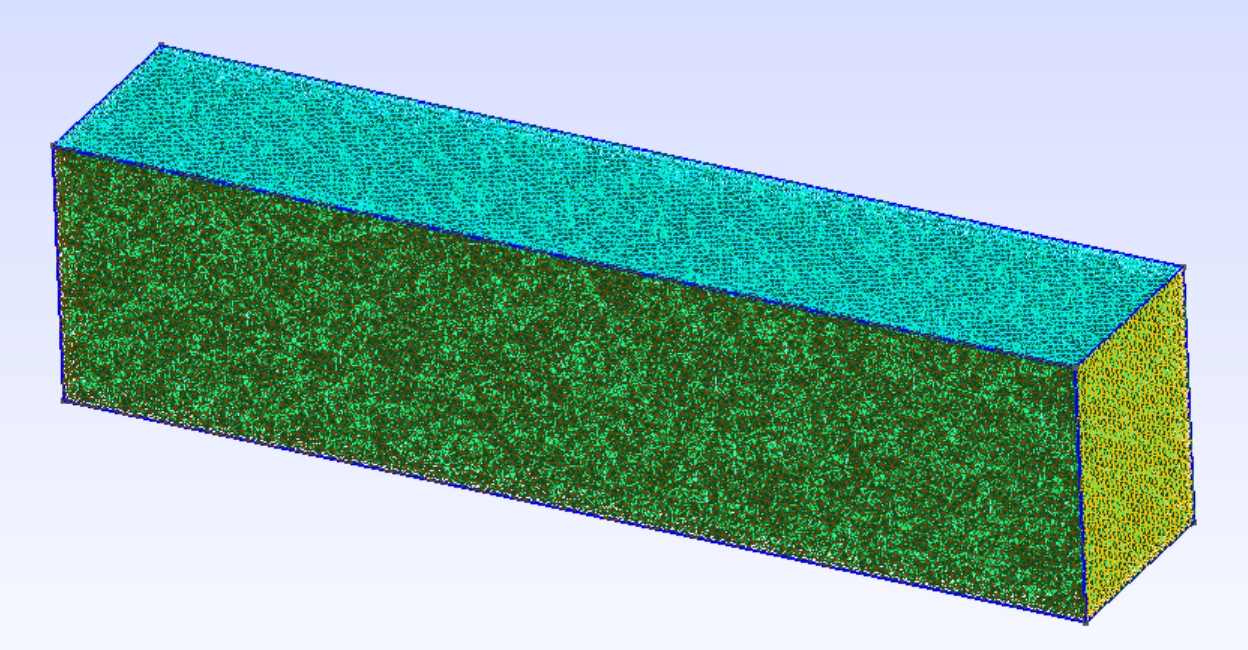
\includegraphics[width=0.5\linewidth]{media/meshing_Q5.png}
        \caption{Finite element meshing using Julia.}
        \label{fig:Julia-3}
    \end{figure}

6(a) Steps for finite element meshing using Abaqus.
    \begin{itemize}
        \item Same step as follow in ~\ref{prob:{5a}}.
    \end{itemize}

    \begin{figure}[H]
        \centering
        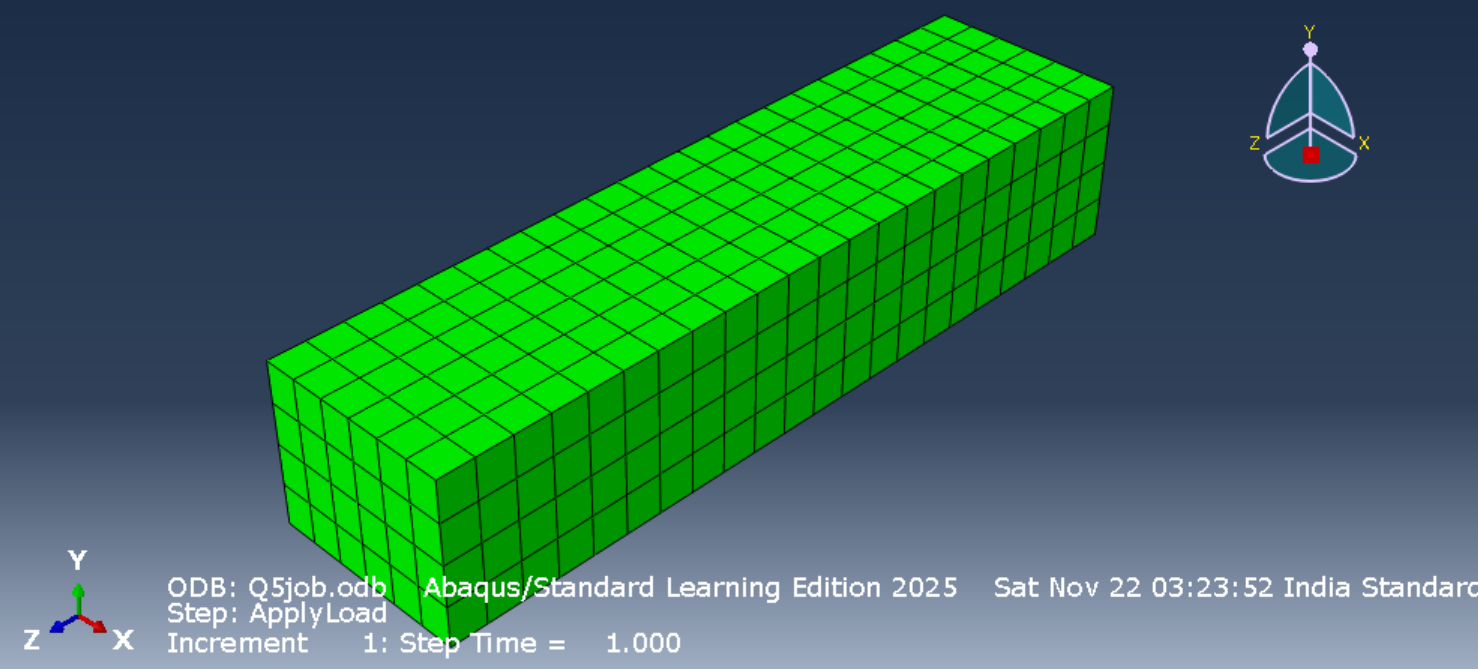
\includegraphics[width=0.5\linewidth]{media/meshing_Q5_Abaqus.png}
        \caption{Finite element meshing using Abaqus.}
        \label{fig:Abaqus-3}
    \end{figure}

    \textbf{Solution: 6}
    (b)  Stress distribution. 
    \sloppy
    \begin{minted}{julia}
        using Gridap
        using GridapGmsh
        
        # 1. Read the Mesh
        model = GmshDiscreteModel("Cantilever_Q6.msh")
        
        # 2. Material Parameters (Steel)
        const E = 25000.0  # MPa
        const ν = 0.2       # Poisson's ratio
        
        # Lamé parameters for Plane Stress
        
        g = VectorValue(0.0,0.0,-1000.0)     ## force
        
        const λ = (E*ν)/((1+ν)*(1-2*ν))
        const μ = E/(2*(1+ν))
        σ(ε) = λ*tr(ε)*one(ε) + 2*μ*ε
        
        # 3. Define FE Spaces
        order = 1
        
        reffe = ReferenceFE(lagrangian,VectorValue{3,Float64},order)
        V0 = TestFESpace(model,reffe;
            conformity=:H1,
            dirichlet_tags=["FixedEnd"],
            dirichlet_masks=[(true,true,true)])
          
        g1 = VectorValue(0.0,0.0,0.0)
        U = TrialFESpace(V0,[g1])
        
        # 4. Numerical Integration
        degree = 2*order
        Ω = Triangulation(model)
        dΩ = Measure(Ω,degree)
        Γ_load  = BoundaryTriangulation(model, tags = "LoadFace")
        dΓ_N = Measure(Γ_load,degree)
        
        # Weak from
        
        # Internal work (Stiffness component)
        a(u,v) = ∫( ε(v) ⊙ (σ∘ε(u)) )*dΩ 
        
        # External Work
        l(v) = ∫(v⋅g)*dΓ_N
        
        # Solve
        op = AffineFEOperator(a,l,U,V0)
        uh = solve(op)
        
        # 7. Post-Process
        writevtk(Ω,"results_Q6",
            cellfields=[
                "Displacement"=>uh,
                "Strain"=>ε(uh),
                "Stress"=>σ∘ε(uh)]
                )
    \end{minted}

    6(c) Comparison between the results obtained from Gridap in Julia and Abaqus.

    \begin{figure}[H]
        \centering
        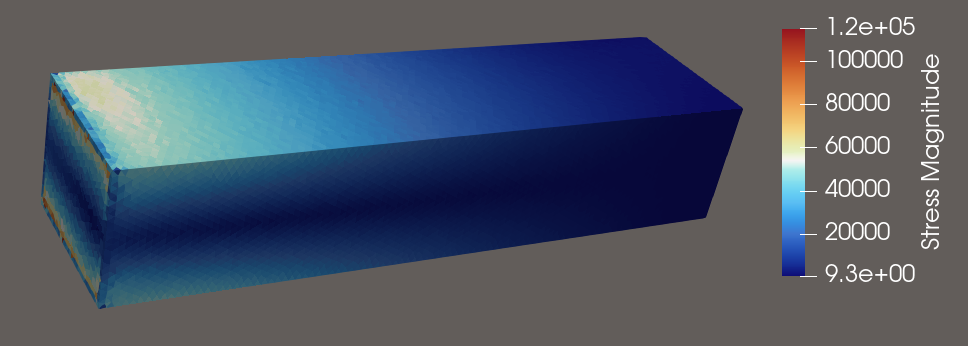
\includegraphics[width=0.5\linewidth]{media/ResultQ6julia.png}
        \caption{Stress distribution using julia}
        \label{fig:ResultQ6julia}
    \end{figure}

    \begin{figure}[H]
        \centering
        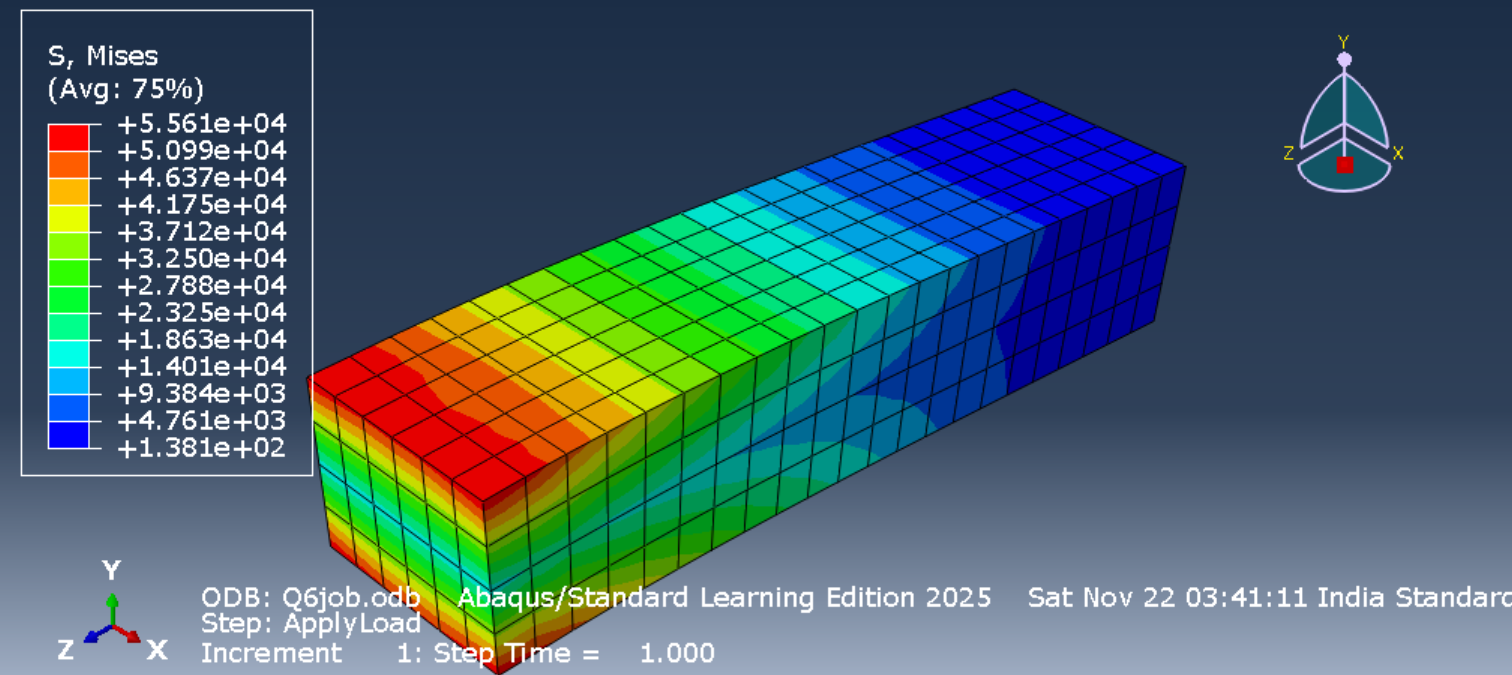
\includegraphics[width=0.5\linewidth]{media/ResultQ6Abaqus.png}
        \caption{Stress distribution using Abaqus}
        \label{fig:ResultQ6Abaqus}
    \end{figure}

    
\end{solution}




% citations
% \bibliographystyle{plain}
% \bibliography{citations.bib}

\vspace{2cm}  % Adds vertical space before the ending line
\begin{center}
    \textbf{-- -- -- The End -- -- --}
\end{center}

\end{document}
